\documentclass[a4paper,11pts]{report}

\usepackage[english]{babel}
\usepackage{color}
\usepackage{amsmath}
\usepackage{graphicx}
\usepackage[a4paper,left=2cm,right=2cm,top=1.5cm,bottom=1.5cm]{geometry}

\begin{document}

\title{SOLEDGE Regression test report}
\date{\today}
\maketitle

\chapter*{Grids}
Examples for $N_r=N_\theta=32$
\begin{table}[!h]
\centering
\begin{tabular}{cc}
  \textbf{Regular grid / Grid1} &   \textbf{Irregular grid / Grid2} \\
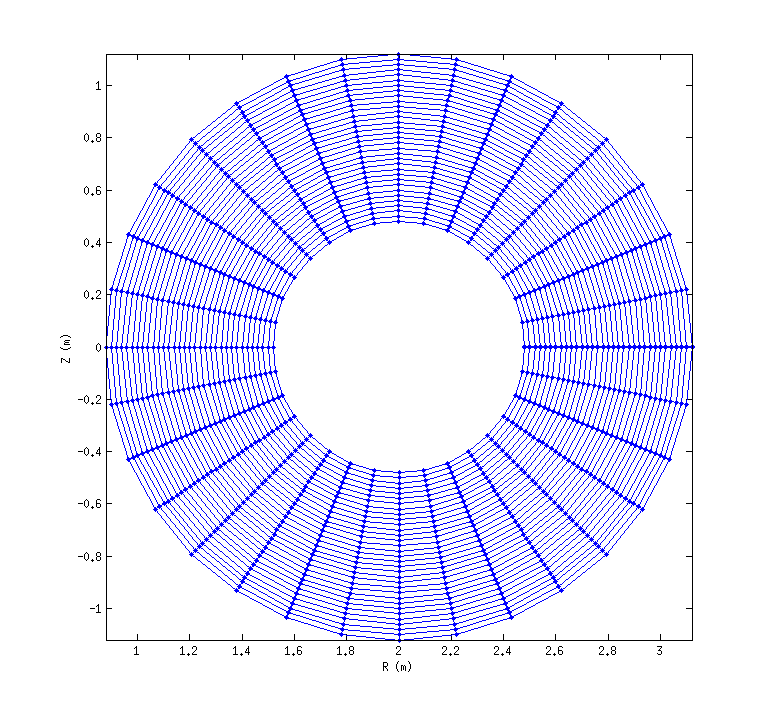
\includegraphics[height=7cm]{grids/regular.png} & 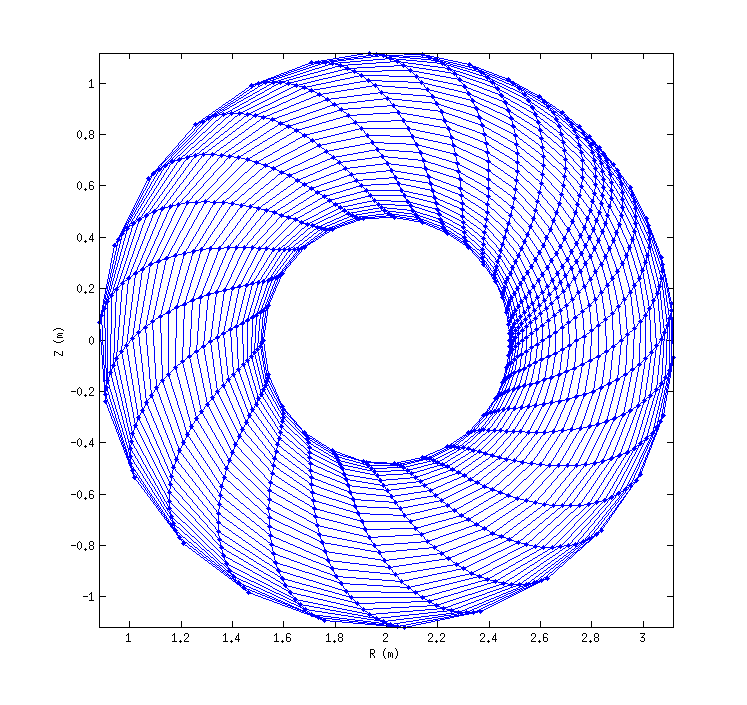
\includegraphics[height=7cm]{grids/irregular.png}
\end{tabular}
\end{table}
\begin{table}[!h]
\centering
\begin{tabular}{c}
  \textbf{Regular twisted grid / Grid3}  \\
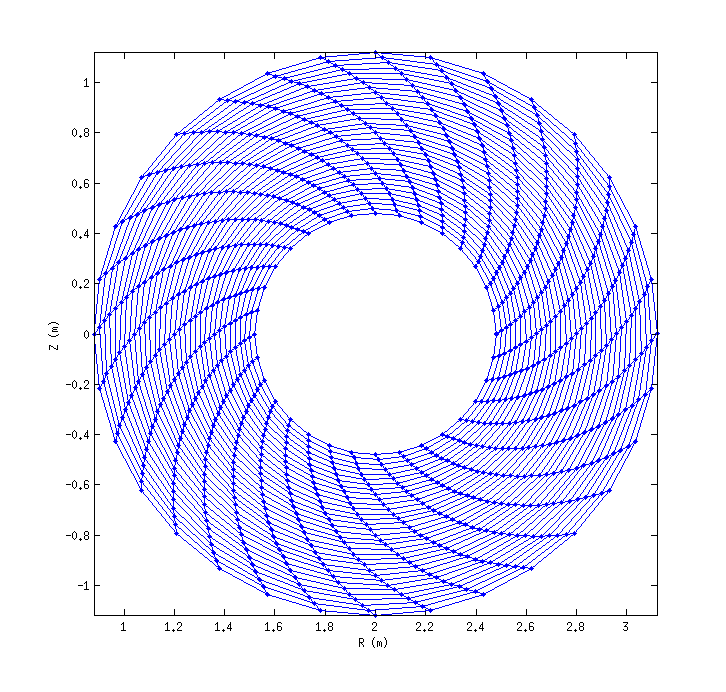
\includegraphics[height=7cm]{grids/regular_twist.png} 
\end{tabular}
\end{table}

\chapter*{Metrics}


  \begin{figure}[!h]
    \centering
    \begin{tabular}{cc}
  \hspace{-1.5cm}      \includegraphics[height=7.5cm]{errors/err_abs_metric_grid1.png} &
      \includegraphics[height=7.5cm]{errors/err_rel_metric_grid1.png}
    \end{tabular}
\caption{Regular grid - Absolute and relative truncation error}
  \end{figure}

  \begin{figure}[!h]
    \centering
    \begin{tabular}{cc}
      \hspace{-1.5cm}      \includegraphics[height=7.5cm]{errors/err_abs_metric_grid3.png} &
      \includegraphics[height=7.5cm]{errors/err_rel_metric_grid3.png}
    \end{tabular}
\caption{Irregular grid - Absolute and relative truncation error}
  \end{figure}


 \newpage

\chapter*{Parallel advection}

System tested:
\begin{equation*}
  \left\{
  \begin{array}{l}
    \partial_t n + \vec{\nabla} \cdot (n v \vec{b}) = 0 \\
    \partial_t (m_i n v) + \vec{\nabla} \cdot (m_i n v^2 \vec{b}) = -\nabla_\parallel (n T) + Z_i n E_\parallel \\
    \partial_t \left( \frac{3}{2} n T + \frac{1}{2} m_i n v^2 \right) + \vec{\nabla} \cdot \left( \frac{5}{2} n T v \vec{b} + \frac{1}{2} m_i n v^3 \vec{b}  \right) = Z_i n v E_\parallel \\
E_\parallel = - \frac{\nabla_\parallel (n T_e)}{n}
  \end{array} \right.
\end{equation*}


  \begin{figure}[!h]
    \centering
    \begin{tabular}{cc}
  \hspace{-1.5cm}      \includegraphics[height=7.5cm]{errors/err_abs_adv_grid1.png} &
      \includegraphics[height=7.5cm]{errors/err_rel_adv_grid1.png}
    \end{tabular}
\caption{Regular grid - Absolute and relative truncation error}
  \end{figure}

  \begin{figure}[!h]
    \centering
    \begin{tabular}{cc}
      \hspace{-1.5cm}      \includegraphics[height=7.5cm]{errors/err_abs_adv_grid2.png} &
      \includegraphics[height=7.5cm]{errors/err_rel_adv_grid2.png}
    \end{tabular}
\caption{Irregular grid - Absolute and relative truncation error}
  \end{figure}

\newpage

\chapter*{Perpendicular diffusion}

System tested:
\begin{equation*}
  \left\{
  \begin{array}{l}
    \partial_t n  =  \vec{\nabla} \cdot (D \vec{\nabla}_\perp n) \\
    \partial_t (m_i n v) = \vec{\nabla} \cdot (m_i D v \vec{\nabla}_\perp n) + \vec{\nabla} \cdot (m_i \nu n \vec{\nabla}_\perp v) \\
    \partial_t \left( \frac{3}{2} n T + \frac{1}{2} m_i n v^2 \right)  =  \vec{\nabla} \cdot \left( \left(\frac{3}{2} T + \frac{1}{2} m_i v^2 \right) D  \vec{\nabla}_\perp n \right) \\
\hspace{3.5cm} + \vec{\nabla}\cdot\left( \frac{1}{2}m_i n \nu \vec{\nabla}_\perp v^2 \right) + \vec{\nabla} \cdot (n \chi \vec{\nabla}_\perp T)
  \end{array} \right.
\end{equation*}


  \begin{figure}[!h]
    \centering
    \begin{tabular}{cc}
  \hspace{-1.5cm}      \includegraphics[height=7.5cm]{errors/err_abs_perp_grid1.png} &
      \includegraphics[height=7.5cm]{errors/err_rel_perp_grid1.png}
    \end{tabular}
\caption{Regular grid - Absolute and relative truncation error}
  \end{figure}

  \begin{figure}[!h]
    \centering
    \begin{tabular}{cc}
      \hspace{-1.5cm}      \includegraphics[height=7.5cm]{errors/err_abs_perp_grid2.png} &
      \includegraphics[height=7.5cm]{errors/err_rel_perp_grid2.png}
    \end{tabular}
\caption{Irregular grid - Absolute and relative truncation error}
  \end{figure}

\newpage

\chapter*{Parallel diffusion}

System tested:
\begin{equation*}
    \partial_t \left( \frac{3}{2} n T + \frac{1}{2} m_i n v^2 \right)  =  \vec{\nabla}\cdot(\kappa^0 T^{5/2} \nabla_\parallel T \vec{b})
\end{equation*}

  \begin{figure}[!h]
    \centering
    \begin{tabular}{cc}
  \hspace{-1.5cm}      \includegraphics[height=7.5cm]{errors/err_abs_para_grid1.png} &
      \includegraphics[height=7.5cm]{errors/err_rel_para_grid1.png}
    \end{tabular}
\caption{Regular grid - Absolute and relative truncation error}
  \end{figure}

  \begin{figure}[!h]
    \centering
    \begin{tabular}{cc}
      \hspace{-1.5cm}      \includegraphics[height=7.5cm]{errors/err_abs_para_grid2.png} &
      \includegraphics[height=7.5cm]{errors/err_rel_para_grid2.png}
    \end{tabular}
\caption{Irregular grid - Absolute and relative truncation error}
  \end{figure}


\newpage

\chapter*{Collisions}

System tested for $\alpha=0$ (electrons - temperature only), $\alpha=1$ ($He^+$) and $\alpha=2$ ($He^{2+}$):
\begin{equation*}
  \left\{
  \begin{array}{l}
    \partial_t n_\alpha = 0 \\
    n_e = \sum_{\alpha=1}^2 Z_\alpha n_\alpha \\
    n_e v_e = \sum_{\alpha=1}^2 Z_\alpha n_\alpha v_\alpha \\
    \partial_t (m_\alpha n_\alpha v_\alpha)  =  Z_\alpha n_\alpha E_\parallel + \sum_{\beta=0}^2 R_{\alpha\beta} \\
    \partial_t \left( \frac{3}{2} n_\alpha T_\alpha + \frac{1}{2} m_\alpha n_\alpha v_\alpha^2 \right)  = \underbrace{Z_\alpha n_\alpha v_\alpha E_\parallel}_{\textrm{part1}} + \underbrace{\vec{\nabla}\cdot \vec{q_\alpha^u}}_{\textrm{part2}} + \underbrace{\sum_{\beta=0}^2 \left( Q_{\alpha\beta} + v_\alpha R_{\alpha\beta} \right)}_{\textrm{part3}}  \\
    \nabla_\parallel (n_e T_e) = - n_e E_\parallel + \sum_{\beta=0}^2 R_{0\beta}
  \end{array} \right.
\end{equation*}

with:
\begin{eqnarray*}
  R_{\alpha\beta} &=& R_{\alpha\beta}^u + R_{\alpha\beta}^T \\
R_{\alpha\beta}^u &=& -0.51 \times \frac{1}{2}\left(\frac{m_\alpha}{m_\beta} + \frac{m_\beta}{m_\alpha} \right) (nm)_{\alpha\beta} \tau_{\alpha\beta}^{-1} (v_\alpha -v_\beta) \\
R_{\alpha\beta}^T &=& -0.71 (nm)_{\alpha\beta} \left(\frac{Z_\alpha^2 T_\alpha^J}{m_\alpha} - \frac{Z_\beta^2 T_\beta^J}{m_\beta} \right)
\end{eqnarray*}
where:
\begin{equation*}
  \tau_{\alpha\beta} = \frac{3 \sqrt{2} \pi^{3/2} \varepsilon_0^2 m_\alpha m_\beta}{n_{\alpha\beta} e^4 Z_\alpha^2 Z_\beta^2 \log \Lambda} \left(\frac{T_\alpha^J}{m_\alpha} + \frac{T_\beta^J}{m_\beta} \right)^{3/2} 
\end{equation*}
\begin{eqnarray*}
n_{\alpha\beta} &=& \frac{2 n_\alpha n_\beta}{n_\alpha+n_\beta} \\
(nm)_{\alpha\beta} &=& \frac{n_\alpha n_\beta}{n_\alpha/m_\alpha+n_\beta/m_\beta} \\
m_{\alpha\beta} &=& \frac{m_\alpha m_\beta}{m_\alpha+m_\beta}
\end{eqnarray*}

The collisional heat flux is given by:
\begin{equation*}
  q_\alpha^u = \sum_\beta 0.71 T_\alpha Z_\alpha^2 \frac{(nm)_{\alpha\beta}}{m_\alpha} (v_\alpha - v_\beta)
\end{equation*}

The exchange term is given by
\begin{eqnarray*}
  Q_{\alpha\beta} &=& Q_{\alpha\beta}^T + Q_{\alpha\beta}^u \\
Q_{\alpha\beta}^T &=& -\frac{3}{2} \frac{(nm)_{\alpha\beta}}{m_{\alpha\beta}} \tau_{\alpha\beta}^{-1} (T_\alpha^J -T_\beta^J) \\
Q_{\alpha\beta}^u &=& -R_{\alpha\beta} (v_\alpha-v_\beta) \frac{m_\beta}{m_\alpha + m_\beta}
\end{eqnarray*}

\newpage
  \begin{figure}[!h]
    \centering
    \begin{tabular}{cc}
  \hspace{-2cm}      \includegraphics[height=7.5cm]{errors/err_abs_col_grid1v.png} &
      \includegraphics[height=7.5cm]{errors/err_rel_col_grid1v.png}
    \end{tabular}
\caption{Regular grid - Absolute and relative truncation error}
  \end{figure}

  \begin{figure}[!h]
    \centering
    \begin{tabular}{cc}
      \hspace{-2cm}      \includegraphics[height=7.5cm]{errors/err_abs_col_grid1T.png} &
      \includegraphics[height=7.5cm]{errors/err_rel_col_grid1T.png}
    \end{tabular}
\caption{Irregular grid - Absolute and relative truncation error}
  \end{figure}

\newpage
  \begin{figure}[!h]
    \centering
    \begin{tabular}{cc}
  \hspace{-2cm}      \includegraphics[height=7.5cm]{errors/err_abs_col_grid2v.png} &
      \includegraphics[height=7.5cm]{errors/err_rel_col_grid2v.png}
    \end{tabular}
\caption{Regular grid - Absolute and relative truncation error}
  \end{figure}

  \begin{figure}[!h]
    \centering
    \begin{tabular}{cc}
      \hspace{-2cm}      \includegraphics[height=7.5cm]{errors/err_abs_col_grid2T.png} &
      \includegraphics[height=7.5cm]{errors/err_rel_col_grid2T.png}
    \end{tabular}
\caption{Irregular grid - Absolute and relative truncation error}
  \end{figure}



\end{document}
